\chapter{Conclusion and Future Works}

This chapter provides a summary of the thesis (Section \ref{thesis_sum}), the challenges(Section \ref{challenge}), and the future work (Section \ref{fw}).

\section{Thesis Summary}\label{thesis_sum}

This project developes a software as a 3D Slicer extension to semi-automatically extract a 3D geometry of the aorta. To build confidence in the software, we applied assurance case arguments. The project started from a Jupyter Notebook program as left by a previous student. With this as a starting point, we explored what changes to the documentation, design, implementation and verification activities are necessary for the assurance case. We did the following tasks in the chronological order for the evidence supporting our assurance case:

\begin{figure}[H]
\fbox{\parbox{\textwidth}{
 \begin{myEnumerate}
\item Build the continuous integration infrastructure with GitHub Actions for the algorithm. This allows us to update the algorithm, and making sure that the valid update is at least as good as the previous version. 
\item A Linter is set up as part of the continuous integration test to ensure the program's readability by enforcing the PEP8 standard.
\item Draft our software requirements specification (SRS).
\item Draft our high-level designs Module Guide (MG).
\item Build a graphical user interface (GUI) because the existing approach had poor usability since it required using other software to determine the necessary parameters and then editing the code.
\item Use 3D Slicer as the platform to implement our GUI because it is modular, and it provides useful features such as Volume Rendering, volume visualization, Crop Volume and reading coordinate on a volume interactively.
\item Build assurance cases in Goal Structuring Notation with the bottom-up approaches. We gather our existing evidence, and explore new implementation requirement for the new evidence.
\item Write user instructions on GitHub README to instruct user use AGR correctly.
\item Film and post a user instructions video with voice over to provide a clear and direct user instructions
\item Build a detailed design document and hosted on a web server.
\item Scheduled Code Review with Kailin
\item Scheduled Algorithm Review with Dr. Dean Inglis.
\item Finalize our SRS, MG, and assurance case. 
\end{myEnumerate}
}}
    \caption[Project List Of Tasks]{Project List Of Tasks}
    \label{fig_contributions}
\end{figure}

It is worth mentioning that GitHub Issues, Discussions, and Pull requests are used throughout the development of the software for the project management. Me and Dr. Spencer Smith were able to keep up good communication through the use of the GitHub features. Finally weekly and bi-weekly meetings were scheduled to help us communicate efficiently.

\section{Challenge}\label{challenge}
In the course of this project, we have summarized a list of challenges. The first challenge was looking for an ideal platform to develop \progname{} software. At the beginning of the project, we wanted to develop our own software without any external platform. Until the point where we see that it is nearly impossible to build from scratch a volume visualization system like the one provided by 3D Slicer, time and efforts have been wasted in design a UI, finding the right tool to build the UI, etc. 

The second challenge is that 3D Slicer itself is a very complex software, the development resource is limited and difficult to understand. Some features provided by 3D Slicer are not as obvious until you have searched through its built-in module list, which has approximately 30 modules.

Another obstacle that we have is having a domain expert to examine the quality of our segmentation result. This medical software's intended user is a university student studying in medical science or medicine, who likes to get an aorta's image or quantified volume. Throughout the development of the \progname{}, we did not have an intended user or a domain expert to review our software. However, me and Dr. Spencer Smith were also lacking the knowledge and do not know the expectation of the intended user, this causes ambiguity to specify the true requirements of AGR.

Finally, it is very challenging of understanding assurance cases within a limited time, and building the assurance cases for AGR was unclear for me. Gathering the evidences and support our arguments was not in my imagination at the beginning of the project, without truely understanding our goals of the project, I was not certain what I was really doing for this project. Until we have several pieces linking together, I was finally understanding and making more efforts in the right direction. 

\section{Future Works}\label{fw}

In this section, we will discuss some possible future works that can continue to make \progname{} better. The first improvement can be done in the segmentation algorithm, and the second improvement involve completing our assurance case.

\subsection{Segmentation Algorithm}

\subsubsection{3D Level Set Approach}
An improved segmentation algorithm \cite{6346433} is available. Like the convention, this algorithm also needs a cropped volume and the aorta seeds to perform segmentation. However, it required less hyperparameters such as the parameters for SimpleITK's ThresholdSegmentationLevelSetsFilter. Using this algorithm will reduce the problem of user inputs, which help to build the evidence for E\_GA.1 discussed in Figure~\ref{fig_agr_ac_ga}.

\subsubsection{Oplique Plane Segmentation}
This algorithm is proposed by Dr. Dean Inglis discussed during our Algorithm Review meeting. This algorithm is based on an assumption, which states that a healthy aorta should have a closer range of diameter. With an initial center coordinate seed and the corresponding diameter, the algorithm can segment the aortic arch through Oblique Plane. Figure~\ref{fig_oblique} shows the double oblique plane in the ascending aorta, and aortic arch.

\begin{figure}[H]
    \centering
    \fbox{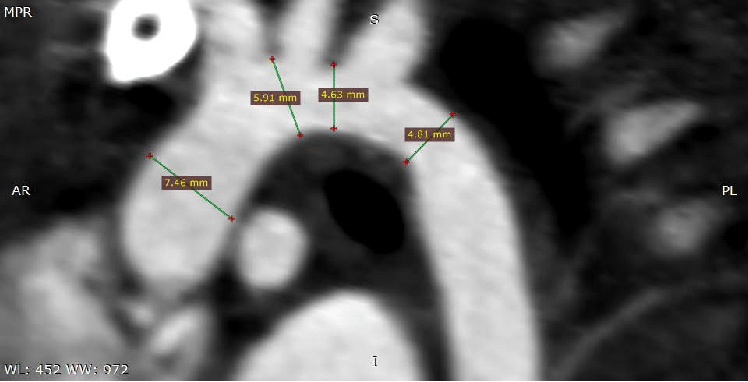
\includegraphics[width=0.8\textwidth]{figures/Conclusion/Ascending-aorta-aortic-arch-and-isthmic-region-in-a-double-oblique-plane-in-a.png}}
    \caption[Aorta Double Oblique Plane]{Aorta Double Oblique Plane}
    \label{fig_oblique}
\end{figure}

\subsection{Assurance Case}

There is room for improvements on the arguments of the requirements of \progname{}. The correctness of the document is reviewed and approved by a domain expert, where there should be evidences that can support the argument. The evidence for  E\_GA.1 discussed in Figure~\ref{fig_agr_ac_ga} is missing because we did not have the time to complete our Verification and Validation Plan (VnV). The VnV should include the test report, an evidence for E\_GA.1, that will indicate if \progname{} throws an exception when the inputs does not meet one or more of the assumptions, with a message that clearly states the reason.